\section{Introduction (2~p)}\label{sec:introduction}

The authors acknowledge support by the state of Baden-Württemberg through \href{https://www.bwhpc.de/}{bwHPC}.

\section{Related Work (3~p)}\label{sec:related-work}

\textbf{Trade Classification in Option Markets}

While classical trade classification algorithms are extensively tested in the stock markets (e.g., \textcite{chakrabartyTradeClassificationAlgorithms2012}; \textcite{odders-whiteOccurrenceConsequencesInaccurate2000}), few works have examined trade classification in option markets.

\textcite[882--883]{savickasInferringDirectionOption2003} are the first to compare the tick rule, quote rule, the Lee and Ready algorithm and the \gls{EMO} rule for options traded at the \gls{CBOE}. The data set spans a period from July 3, 1995 - December 31, 1995 consisting of $869{,}217$ matched trades. The authors report the highest accuracies for the quote rule (\SI{78.98}{\percent}) and find that all rules perform worst when applied to index options. In general, the trade classification rules exhibit significantly lower classification accuracies on options data than with stock data, urging the need for improved classifiers.

The most exhaustive study is the one of \textcite[1--39]{grauerOptionTradeClassification2022}.  The authors test the accuracy of the classical quote rule and tick rule, and hybrids thereof on two large-scale data sets spanning a period from 2005 - 2017. Consistently for options traded at the  \gls{ISE} and \gls{CBOE} classical rules like the popular Lee and Ready algorithm only achieve accuracies of \SI{62.53}{\percent} or \SI{62.03}{\percent} and are thus significantly smaller than in the stock market. In line with the research of  \textcite[886]{savickasInferringDirectionOption2003}, the reported accuracies are inversely proportional to the rule's reliance on past transaction prices. In particular, the tick rule performs worst with accuracies marginally different from a random guess. Overall, the reported success rates deteriorate between both studies and over time. As a remedy, \textcite[14--17]{grauerOptionTradeClassification2022} introduce two additional rules based on the trade and quote sizes. The \textit{depth rule} is an alternative to the tick rule for classifying mid spread trades in the Lee and Ready algorithm and \gls{EMO} rule. It assigns the aggressor of the trade based on the depth at the bid or ask. Together with the \textit{trade size rule}, their second rule, which classifies trades with a trade size matching the size of the bid or ask quote, can substantially improve the performance of classical algorithms. The ensemble of rules achieves an accuracy between \SI{73}{\percent} and \SI{75}{\percent} surpassing previous rules by more than \SI{10}{\percent}, at the cost of data efficiency.

The work of \textcite{grauerOptionTradeClassification2022} is important in two ways. First, the data set is identical to ours, which enables a fair comparison between classical rules and machine learning-based predictors. Second, their stacked combinations of the trade size rule, depth rule, and common trade classification algorithms achieve state-of-the-art performance in option trade classification and are thus a rigorous benchmark.

\textbf{Trade classification using machine learning}

\textcite[5]{rosenthalModelingTradeDirection2012} bridges the gap between classical trade classification and machine learning by fitting a logistic regression model on lagged and unlagged predictors inherent to the tick rule, quote rule, and \gls{EMO} algorithm, as well as a sector-specific and a time-specific term. Instead of using the rule's discretized outcome as a feature, \textcite[481-482]{rosenthalModelingTradeDirection2012} models the rules through so-called information strength functions. The proximity to the quotes, central to the \gls{EMO} algorithm, is thus modelled by a proximity function. Likewise, the information strength of the quote and tick rule is estimated as the log return between the trade price and the midpoint or the previous trade price. However, it only improves the accuracy of the \gls{EMO} algorithm by a marginal \SI{2}{\percent} for Nasdaq stocks and \SI{1.1}{\percent} for \gls{NYSE} stocks \textcite[15]{rosenthalModelingTradeDirection2012}. Our work aims to improve the model by exploring non-linear estimators and minimizing data modelling assumptions.

The work of \textcite[483]{blazejewskiLocalNonParametricModel2005} compares a $k$-nearest neighbour classifier against logistic regression, as well as simple heuristics like the majority vote over past trades for signing trades at the Australian stock exchange. Their results indicate that the parametric $k$-nearest neighbour classifier improves upon a linear logistic regression in terms of classification accuracy, even when trained on fewer features. The work is unique from the remaining works about feature set definition. Notably, \textcite[3]{blazejewskiLocalNonParametricModel2005} use no quote or trade prices, but rather the order book volumes, trade sizes, and past trade signs for classification. No accuracies for classical trade signing rules are reported, which impedes a comparison across different works. In line with their results, we focus on non-linear models in the form of gradient boosting and transformers. Additionally, our paper addresses the mentioned shortcomings by benchmarking against state-of-the-art trade classification rules. We share the idea of using the trade size, as well as the bid and ask sizes for classification for some of our feature sets, but greedily predict using non-historic features.

Closest to our work is a publication of \textcite[1--58]{ronenMachineLearningTrade2022}. Therein, the authors compare a selection of machine learning algorithms against classical trade signing rules in the bond and stock market. Their comparison is the first to consider both logistic regression, a random forest, as well as feed-forward networks. Over a wide range of feature sets the tree-based ensemble consistently outperforms by out-of-sample accuracy the tick rule and Lee and Ready algorithm, as well as all remaining machine learning models. For the TRACE and ITCH data set, their best variant of the random forest outperforms the tick rule by \SI{8.3}{\percent} and \SI{3.3}{\percent}, respectively \autocite[57]{ronenMachineLearningTrade2022}. Whilst the superiority of random forests is consistent for the bond and equity market, fitted classifiers do not transfer across markets, as diminishing accuracies for the transfer learning by model transfer indicate.

The results convincingly demonstrate the potential of machine learning, i.e., of tree-based ensembles, for trade classification. Yet, the comparability of the results is limited by the classifier's reliance on additional features beyond quote and price data. Albeit, \textcite[4]{ronenMachineLearningTrade2022} consider a wide range of approaches, their selection leaves the latest advancements in artificial neural networks and ensemble learning aside and is mainly guided by computational constraints. Even if the focus is on standard techniques, the unclear research agenda concerning model selection, tuning, and testing hampers the transferability of their results to the yet unstudied option market.

In summary, machine learning has been applied successfully in the context of trade classification. To the best of our knowledge, no previous work perform machine learning-based classification in the options markets.

\newpage
\section{Rule-Based Approaches (5.5~p)}\label{sec:rule-based-approaches}


% The following section introduces common rules for signing option trades. We start by introducing the classical quote and tick rule and continue with the more recent depth and trade size rule. In section \ref{hybrid-rules} we combine some rules from section \ref{basic-rules} to hybrids thereof. We conclude this chapter by drawing a connection to ensemble learning.

\subsection{Basic Rules (3~p)}\label{sec:basic-rules}

% Starting with the quote rule, we describe the most common rule for signing option trades, which can either be used as-is or joint in more complex rules.

\subsubsection{Quote Rule (0.75~p)}\label{sec:quote-rule}

The quote rule compares the trade price against the corresponding quotes at the time of the trade. If the trade price $p_{i,t}$ is above the midpoint of the bid-ask spread, denoted by $m_{i,t} = \tfrac{1}{2}(b_{i,t} + a_{i,t})$, the trade is classified as a buy and if it is below the midpoint, as a sell \autocite[][41]{harrisDayEndTransactionPrice1989}. Thus, the classification rule on $D = \left\{(p_{i,t}, m_{i,t}) \in \mathbb{R}^2: p_{i,t} \neq m_{i,t}\right\}$ is given by:

\begin{equation}
  \operatorname{quote}\colon D \to \left\{0, 1\right\},\quad
  \operatorname{quote}(p_{i,t}, m_{i,t})=
  \begin{cases}
    0, & \text{if}\ p_{i, t}>m_{i, t}  \\
    1, & \text{if}\ p_{i, t}<m_{i, t}. \\
  \end{cases}
\end{equation}

By definition, the quote rule cannot classify trades at the midpoint of the quoted spread. \textcite[][241]{hasbrouckTradesQuotesInventories1988} discusses multiple alternatives for signing mid-spread trades based on the subsequent quotes, contemporaneous, or the subsequent transaction. However, the most common approach to overcome this limitation is, to combine the quote rule with other approaches, such as the tick rule, into an ensemble.

The quote rule requires to match one bid and ask quotes with each trade based on a timestamp. Due to the finite resolution of the dataset's timestamps and active markets, multiple quote changes can co-occur at the time of the trade, some of which, are actually after the trade. As such, it remains unclear which quote to consider in trade classification, and a quote timing technique must be employed. Empirically, \textcite[][1765]{holdenLiquidityMeasurementProblems2014} observe, that the most common choice is to use the last quote by order from the time increment (e.g., the second) before the trade.

In contrast to the tick rule, the quote rule requires both trade price and quote data, and is thus less data efficient. The reduced dependence on past transaction prices and the focus on quotes has nonetheless positively impacted classification accuracies in option markets, as the studies of \textcite[][886]{savickasInferringDirectionOption2003} and \textcite[][3]{grauerOptionTradeClassification2022} reveal. Especially, if trade classification is performed on the NBBO.


\subsubsection{Tick Test (0.75~p)}\label{sec:tick-test}

Based on the rationale that buys increase the trade price and sells lower them, the tick test classifies trades by the change in trade price \autocite[][271]{easleyDiscerningInformationTrade2016}. Its was first applied in \textcites[][244]{holthausenEffectLargeBlock1987}[][240]{hasbrouckTradesQuotesInventories1988}.

The tick test, $\operatorname{tick}\colon \mathbb{R}^2 \to \left\{0,1\right\}$, is formally defined as:

\begin{equation}
  \operatorname{tick}(p_{i, t-1}, p_{i,t})=
  \begin{cases}
    1,                                         & \text{if}\ p_{i, t} > p_{i, t-1} \\
    0,                                         & \text{if}\ p_{i, t} < p_{i, t-1} \\
    \operatorname{tick}(p_{i,t-2}, p_{i,t}), & \text{else}.
  \end{cases}
  \label{eq:tick-test}
\end{equation}


Considering the cases in \cref{eq:tick-test} the trade price is higher than the previous price (uptick) the trade is classified as a buy. Reversely, if it is below the previous price (downtick), the trade is classified as a sell. If the price change is zero (zero tick), the signing uses the last price different from the current price. \autocite[][3]{leeInferringTradeDirection1991}

By this means, the tick rule can sign all trades as long as there is a last distinguishable trade price, but the overall precision can be impacted for infrequently traded assets. Being only dependent on transaction data makes the tick rule highly data-efficient. Waiving any quote data for classification contributes to this efficiency, but also poses a major limitation with regard to trades at the bid or ask, as discussed in \textcite[][557--558]{finucaneDirectTestMethods2000}. For instance, if quotes rise between trades, then a sale at the bid on an uptick or zero uptick, is misclassified as a buy by tick test due to the overall increased trade price. Similarly for falling quotes, buys at the ask on downticks or zero downticks are erroneously classified as a sell.

The reverse tick test is a variant of the tick test is the reverse tick test as applied in \textcite[][241]{hasbrouckTradesQuotesInventories1988}. It is similar to the tick rule but classifies based on the trade price of the next, distinguishable trade price. As donated in \cref{eq:tick-test} the trade is classified as seller-initiated, if the next trade is on an uptick or a zero uptick, and classified as buyer-initiated for trades at a downtick or a zero downtick \autocite[][735--636]{leeInferringTradeDirection1991}.

\begin{equation}
  \operatorname{rtick} \colon \mathbb{R}^2 \to \left\{0, 1\right\}, \quad \operatorname{rtick}(p_{i, t}, p_{i,t+1})=
  \begin{cases}
    1,                     & \text{if}\ p_{i, t} > p_{i, t+1} \\
    0,                     & \text{if}\ p_{i, t} < p_{i, t+1} \\
    \operatorname{rtick}(p_{i,t}, p_{i,t+2}), & \text{else}
  \end{cases}
  \label{eq:reverse-tick-test}
\end{equation}

Both the tick test and reverse tick test result in the same classification, if the current trade is bracketed by a price reversal and the price change after the trade is opposite from the change before the trade, but differ for price continuations when price changes are in the same direction \autocite[][736]{leeInferringTradeDirection1991}. In practice, \textcite[][29--32]{grauerOptionTradeClassification2022} observe higher accuracies for the reverse tick test on a sample of option trades recorded at the \gls{ISE} and \gls{CBOE}. This result contradicts results in the stock market \textcite[][737]{leeInferringTradeDirection1991}. Lags behind quote based classification.

\subsubsection{Depth Rule (0.75~p)}\label{sec:depth-rule}

As the \cref{sec:quote-rule} unveils, the tick rule yields significantly lower success rates than the quote rule. For midspread trades, that can otherwise not be classified by the advantageous quote rule, \textcite[][14]{grauerOptionTradeClassification2022} propose the depth rule.

The depth rule infers the trade initiator from the quoted size at the best bid and ask. Based on the observation that an exceeding bid or ask size relates to higher liquidity on one trade side, trades are classified as a buy for a larger ask size and sell for a higher bid size \textcite[][14]{grauerOptionTradeClassification2022}.

Let $\tilde{a}_{i,t}$ denote the quoted size of the ask and $\tilde{b}_{i,t}$ of the bid. We set the domain as $D = \left\{(p_{i,t}, m_{i,t}, \tilde{a}_{i,t}, \tilde{b}_{i,t}) \in \mathbb{R}^4: p_{i,t} = m_{i,t} \ \text{and} \ \tilde{a}_{i,t} \neq \tilde{b}_{i,t} \right\}$. The depth rule, $\operatorname{depth} \colon D \to \left\{0,1\right\}$, is now defined as:
\begin{equation}
  \operatorname{depth}(p_{i,t}, m_{i,t}, \tilde{a}_{i,t}, \tilde{b}_{i,t})=
  \begin{cases}
    0, & \tilde{a}_{i,t} < \tilde{b}_{i,t} \ \text{and}\ p_{i, t} = m_{i, t} \\
    1, & \tilde{a}_{i,t} > \tilde{b}_{i,t} \ \text{and}\ p_{i, t} = m_{i, t}. \\
  \end{cases}
  \label{eq:depth-rule}
\end{equation}

As shown in \cref{eq:depth-rule}, the depth rule classifies midspread trades only, if the ask size is different from the bid size, as the ratio between the ask and bid size is the sole criterion for inferring the trade's aggressor. Due to these restrictive conditions, the depth rule can only sign a small fraction of all trades and is best stacked with others rules.

Like the quote rule, the depth rule has additional dependencies on quote data. Despite being applied to midpoint trades only, \textcite[][4]{grauerOptionTradeClassification2022} report an improvement in the overall accuracy \SI{1.2}{\percent} for the  \gls{CBOE} data set and by \SI{0.8}{\percent} on the  \gls{ISE} sample merely through the depth rule. The rule has not yet been tested in other markets.

\subsubsection{Trade Size Rule (0.75~p)}\label{sec:trade-size-rule}

As the \cref{sec:quote-rule} derives, quote-based approaches are generally preferred due to the improved performance relative to the tick test. \textcite[][13]{grauerOptionTradeClassification2022} stress that the quote rule, however, systematically misclassifies limit orders and propose an alternative procedure to identify and override predictions for them. On the domain $D = \left\{(\tilde{p}_{i, t} , \tilde{a}_{i, t} , \tilde{b}_{i,t}) \in \mathbb{R}^3: \tilde{p}_{i,t} = \tilde{a}_{i,t} \neq \tilde{b}_{i,t} \ \text{or} \ \tilde{p}_{i,t} \neq  \tilde{a}_{i,t} = \tilde{b}_{i,t} \right\}$ the trade size rule, $\operatorname{tsize} \colon D \to \left\{0,1\right\}$, is defined as:
\begin{equation}
  \operatorname{tsize}(\tilde{p}_{i, t} , \tilde{a}_{i, t} , \tilde{b}_{i,t})=
  \begin{cases}
    1, & \text{if}\ \tilde{p}_{i, t} = \tilde{b}_{i, t} \neq \tilde{a}_{i, t} \\
    0, & \text{if}\ \tilde{p}_{i, t} = \tilde{a}_{i, t} \neq \tilde{b}_{i, t}. \\
  \end{cases}
  \label{eq:trade-size-rule}
\end{equation}

The trade size rule in \cref{eq:trade-size-rule} classifies based on a match between the size of the trade $\tilde{p}_{i, t}$ and the quoted bid and ask sizes. The rationale is, that the market maker tries to fill the limit order of a customer, which results in the trade being executed at the prevailing bid or ask, with a trade size equalling the quoted size \textcite[][13]{grauerOptionTradeClassification2022}. By definition, when both the size of the ask and bid correspond with the trade size, no class can be assigned.

\textcite[][13]{grauerOptionTradeClassification2022} report an accuracy of \SI{79.92}{\percent} for the subset of option trades at the  \gls{ISE} (\SI{22.3}{\percent} of all trades) that can be signed using the methodology, which contributes to a performance improvement of \SI{11}{\percent} for the entire sample. Expectedly, the improvement is highest for trades at the quotes and reverses for trades outside the quote \textcite[][15]{grauerOptionTradeClassification2022}. Based on these results, the trade size rule may only be applied selectively to trades inside or at the quote. Since only a fraction of all trades can be classified with the trade size rule, the rule must be combined with other basic or hybrid rules for complete coverage. The subsequent section introduces three such hybrid algorithms, that combine the tick and quote rule into more sophisticated algorithms to address the limitations of the former.

\subsection{Hybrid Rules (2.5~p)}\label{sec:hybrid-rules}

\subsubsection{Lee and Ready Algorithm (1 p)}\label{sec:lee-and-ready-algorithm}

The popular \gls{LR} algorithm combines the (reverse) tick test and quote rule into a single algorithm. The algorithm signs trades according to the quote rule trades. Trades at the midpoint of the spread, which cannot be classified with the quote rule, are classified with the tick rule and quote rule, the \gls{LR} algorithm can thus be defined as:

\begin{equation}
  \operatorname{lr} \colon \mathbb{R}^3 \to \left\{0,1\right\}, \quad
  \operatorname{lr}(p_{i,t-1}, p_{i,t}, m_{i,t})=
  \begin{cases}
    1,                                       & \text{if}\ p_{i, t} > m_{i, t} \\
    0,                                       & \text{if}\ p_{i, t} < m_{i, t} \\
    \operatorname{tick}(p_{i,t-1}, p_{i,t}), & \text{else}.
  \end{cases}
\end{equation}

The strength of the algorithm lies in combining the strong classification accuracies of the quote rule with the universal applicability of the tick test. As it requires both trade and quote data, it is less data-efficient than its parts.


\subsubsection{Ellis-Michaely-O'Hara
  Rule (0.75~p)}\label{sec:ellis-michaely-ohara-rule}

\textcite[][536]{ellisAccuracyTradeClassification2000} examine the performance of the previous algorithms for stocks traded at NASDAQ. By analyzing miss-classified trades with regard to the proximity of the trade to the quotes, they observe, that the quote rule and by extension of the \gls{LR} algorithm performs particularly well at classifying trades executed at the bid and the ask price but trail the performance of the tick rule for trades inside or outside the spread \autocite[][535--536]{ellisAccuracyTradeClassification2000}. The authors combine these observations into a single rule, known as the \gls{EMO} algorithm.

As such, the \gls{EMO} algorithm \autocite[][540]{ellisAccuracyTradeClassification2000} extends the tick rule by classifying trades at the quotes using the quote rule, and all other trades with the tick test. Formally, the classification rule is given by:

\begin{equation}
  \operatorname{emo} \colon \mathbb{R}^4 \to \left\{0, 1 \right\}, \quad
  \operatorname{emo}(p_{i, t-1}, p_{i, t}, a_{i, t}, b_{i, t})=
  \begin{cases}
    1,                                         & \text{if}\ p_{i, t} = a_{i, t} \\
    0,                                         & \text{if}\ p_{i, t} = b_{i, t} \\
    \operatorname{tick}(p_{i, t-1}, p_{i, t}), & \text{else}.
  \end{cases}
  \label{eq:emo-rule}
\end{equation}

\Cref{eq:emo-rule} embeds both the quote and tick rule. As trades off the quotes are classified by the tick rule, the algorithm's overall success rate is dominated by the tick test. For option markets \autocites[cp.][891]{savickasInferringDirectionOption2003}[][21]{grauerOptionTradeClassification2022} this dependence caused the performance to lag behind quote-based approaches, contrary to the successful adaption in the stock market \autocites[cp.][541]{ellisAccuracyTradeClassification2000}[][3818]{chakrabartyTradeClassificationAlgorithms2007}. In \textcite[][31--35]{grauerOptionTradeClassification2022} the authors achieve minor improvements in classification accuracy on option exchange data by applying the reverse tick test as a proxy for the tick test.

\subsubsection{Chakrabarty-Li-Nguyen-Van-Ness
  Method (0.75~p)}\label{sec:chakarabarty-li-nguyen-van-ness-method}

Like the previous two algorithms, the \gls{CLNV} method \autocite[][3809]{chakrabartyTradeClassificationAlgorithms2012} is a hybrid of the quote and tick rule and extends the \gls{EMO} rule by a fragmented treatment of trades inside the quotes, which are notoriously hard to classify. \textcite[][3809]{chakrabartyTradeClassificationAlgorithms2012} segment the spread into ten equal-width bins and classify trades around the midpoint (4th - 7th decile) by the tick rule and trades close to the quotes \gls{EMO} rule trades outside the quotes are categorized by the tick rule.

\begin{equation}
  \begin{aligned}
  &\operatorname{clnv} \colon \mathbb{R}^4 \to \left\{0, 1 \right\}\\
  &\operatorname{clnv}(p_{i, t-1}, p_{i, t}, a_{i, t}, b_{i, t})=
  \begin{cases}
    1,                     & \text{if}\ p_{i, t} \in \left(\frac{3}{10} b_{i,t} + \frac{7}{10} a_{i,t}, a_{i, t}\right] \\
    0,                     & \text{if}\ p_{i, t} \in \left[ b_{i,t}, \frac{7}{10} b_{i,t} + \frac{3}{10} a_{i,t}\right) \\
    \operatorname{tick}(p_{i, t-1}, p_{i, t}), & \text{else}
  \end{cases}
  \end{aligned}
  \label{eq:CLNV-rule}
\end{equation}

The algorithm, as summarized in \cref{eq:CLNV-rule}, is derived from a performance comparison of the tick rule / \gls{EMO} rule against the quote rule / \gls{LR} algorithm on stock data, whereby the accuracy was assessed separately for each decile \footnote{The spread is assumed to be positive and evenly divided into ten deciles and the 1st to 3rd deciles are classified by the quote rule. Counted from the bid, the first decile starts at $b_{i,t}$ and  $b_{i,t} + \tfrac{3}{10} (a_{i,t} - b_{i,t}) = \tfrac{7}{10} b_{i,t} + \tfrac{3}{10} a_{i,t}$ marks the beginning of the 3rd decile. As all trade prices are below the midpoint, they are classified as a sell.}. The classical \gls{CLNV} method uses the backward-looking tick rule. In the spirit of \textcite[][735]{leeInferringTradeDirection1991}, the tick test could be replaced by the reverse tick test.


\textcite[][3811]{chakrabartyTradeClassificationAlgorithms2007} continue the trend for more complex classification rules, leading to a higher fragmented decision surface, and eventually resulting in improved classification accuracy. Since the decision, which of the base rules is applied, is inferred from \emph{static} cut-off points at the decile boundaries of the spread -- including the midspread and the quotes -- current classification rules may not realize their full potential. A obvious question is, if classifiers, \emph{learned} on price and quote data, can adapt to the data and thereby improve over traditional trade classification rules.

The trend towards sophisticated, hybrid rules, sometimes combining as many as four base rules into a single classifier \autocite[cp.][18]{grauerOptionTradeClassification2022}, has conceptual parallels to (stacked) ensembles found in machine learning and expresses the need for better classifiers. In the subsequent section, we provide an overview of state-of-the-art machine learning approaches for classification. We start by framing trade classification as a supervised learning problem.
\newpage
\section{Supervised Approaches (12~p)}\label{sec:supervised-approaches}

\subsection{Selection of Approaches (2~p)}\label{sec:selection-of-approaches}

\subsection{Gradient Boosted Trees (2~p)}\label{sec:gradient-boosted-trees}

\subsubsection{Decision Tree (0.5~p)}\label{sec:decision-tree}

\subsubsection{Gradient Boosting
  Procedure (1.5 p)}\label{sec:gradient-boosting-procedure}

\subsection{Transformer Networks}\label{sec:transformer-networks}

\subsubsection{Architectural Overview}\label{sec:architectural-overview}

\begin{landscape}
  \begin{figure}
    \begin{center}
      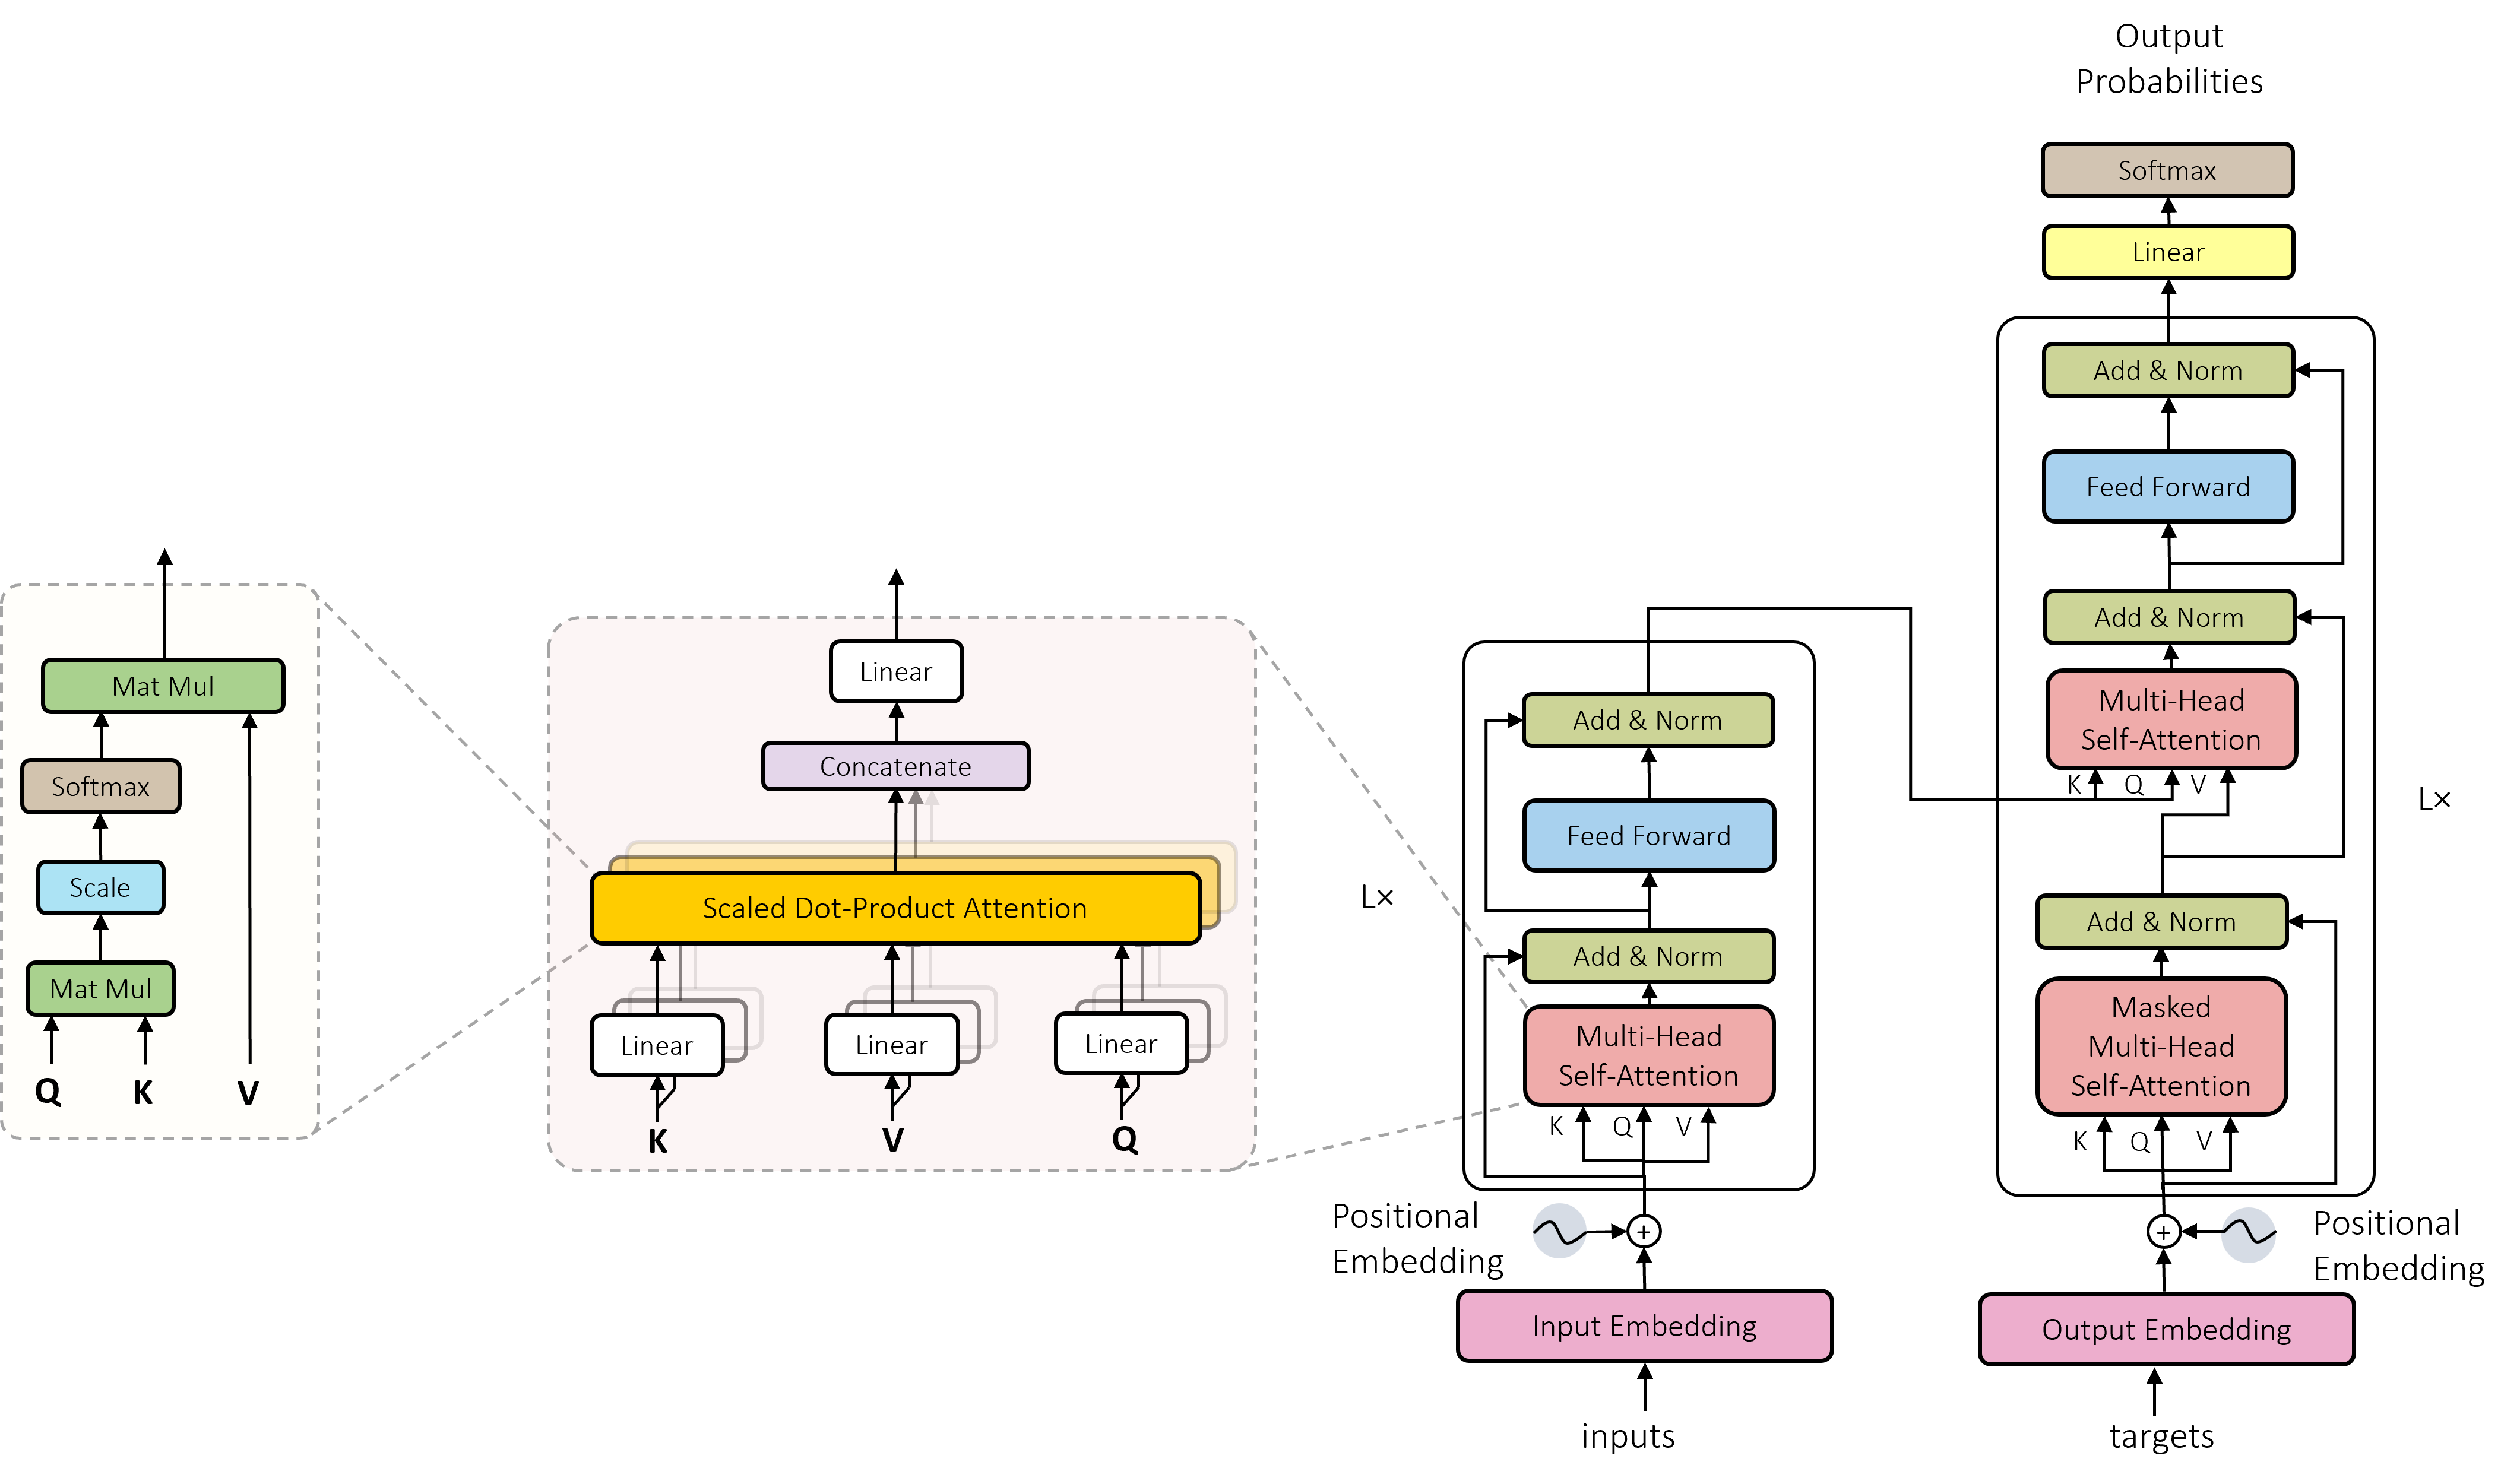
\includegraphics[width=\textwidth]{classical_transformer}
    \end{center}
    \caption{Own drawing inspired by \textcite{daiTransformerXLAttentiveLanguage2019}}
  \end{figure}
\end{landscape}

\subsubsection{Token Embedding}\label{sec:token-embeddings}

\subsubsection{Positional Encoding}\label{sec:positional-encoding}

\subsubsection{Attention}\label{sec:attention}

\subsubsection{Position-wise Feed-Forward Networks}\label{sec:position-wise-ffn}

\subsubsection{Residual Connections}\label{sec:residual-connections}

\subsubsection{Layer Normalization}\label{sec:layer-norm}

\subsection{Transformer Networks For Tabular Data}\label{sec:tabular-transformer}

\subsubsection{Tabular Embeddings}\label{sec:tabular-embeddings}

\subsubsection{TabTransformer}\label{sec:tabtransformer}

\subsubsection{FTTransformer}\label{sec:fttransformer}


\newpage
\section{Semi-Supervised Approaches (8~p)}\label{sec:semi-supervised-approaches}

\subsection{Selection of Approaches (2~p)}\label{sec:selection-of-approaches-1}

\subsection{Extensions to Gradient Boosted
  Trees (2~p)}\label{sec:extensions-to-gradient-boosted-trees}

\subsection{Extensions to TabTransformer (2~p)}\label{sec:extensions-to-tabtransformer}

\subsection{Extensions to FTTransformer (2~p)}\label{sec:extensions-to-fttransformer}


\newpage
\section{Empirical Study (19.5~p)}\label{sec:empirical-study}

\subsection{Environment (0.5~p)}\label{sec:environment}

\subsection{Data and Data Preparation (6 p)}\label{sec:data-and-data-preparation}

\subsubsection{ISE Data Set (0.5~p)}\label{sec:ise-data-set}

\subsubsection{CBOE Data Set (0.5~p)}\label{sec:cboe-data-set}

\subsubsection{Exploratory Data Analysis (2~p)}\label{sec:exploratory-data-analysis}

\subsubsection{Data Pre-Processing (1~p)}\label{sec:data-preprocessing}

\subsubsection{Feature Engineering (1.5~p)}\label{sec:feature-engineering}

\subsubsection{Train-Test Split (0.5~p)}\label{sec:train-test-split}

\subsection{Training and Tuning (10~p)}\label{sec:training-and-tuning}

\subsubsection{Training of Supervised
  Models (4~p)}\label{sec:training-of-supervised-models}


\subsubsection{Training of Semi-Supervised
  Models (4~p)}\label{sec:training-of-semi-supervised-models}


\subsubsection{Hyperparameter Tuning (2~p)}\label{sec:hyperparameter-tuning}


\subsection{Evaluation (3~p)}\label{sec:evaluation}

\subsubsection{Feature Importance
  Measure (2~p)}\label{sec:feature-importance-measure}

\subsubsection{Evaluation Metric (1~p)}\label{sec:evaluation-metric}

\newpage
\section{Results (12~p)}\label{sec:results}

\subsection{Results of Supervised
  Models (2~p)}\label{sec:results-of-supervised-models}

\subsection{Results of Semi-Supervised
  Models (2~p)}\label{sec:results-of-semi-supervised-models}

\subsection{Robustness of Results (3~p)}\label{sec:robustness-checks}

\subsection{Feature Importance (3~p)}\label{sec:feature-importance}

\subsection{Ablation Study of Models (2~p)}\label{sec:ablation-study}

\newpage
\section{Application in Transaction Cost Estimation (optional)}\label{sec:application}
\subsection{Simulation Setup (optional)}\label{sec:simulation-setup}
\subsection{Simulation Results (optional)}\label{sec:simulation-results}

\newpage
\section{Discussion (3~p)}\label{sec:discussion}

\newpage
\section{Conclusion (2~p)}\label{sec:conclusion}

\newpage
\section{Outlook (0.5~p=67.5~p)}\label{sec:outlook}

